\lab{Applications}{Balanced Trees}{Balanced Trees}
\label{lab:btrees}

Trees are very versatile structures.  
Their worst case complexity of $O(\log n)$ for inserting, deleting, and searching make them an attractive option when working with lots of data.
In most cases, a simple binary search tree is sufficient.
However, there are cases when we lose all the benefits of a binary search tree.
One example is adding already sorted or nearly sorted data to a binary search tree.
This results in a degnerate BST that performs no better than a linked list!
Another problem is adding more levels to the tree than is necessary.
The more levels a tree has, the less performant it becomes.  If we could somehow fill a level or make it as close to full as possible, we can minimize the number of levels a a search tree has.

\begin{problem}
Write methods to determine the number of levels a tree has and how full each level is.  Look at breadth first search for inspiration on how to accomplish this.
\end{problem}

\section*{Balancing Trees}
There have been a variety of attempts at optimizing the structure of a binary tree.
The method that we will describe in depth is and AVL balanced tree.
AVL trees use the strictest definition of balance.
Another commonly used balanced binary tree is a red-black tree.  AVL trees optimize frequent lookups while red-black trees optimize insertion/deletion performance.
Red-black trees color nodes red or black and check for imbalance based on colors.  For example, a subtree is unbalanced if a red node has a red child.
AVL trees determine balance by comparing the height of right and  left subtrees.
The height of a node is a measure of how far up the tree the node is from the base.
There are four ways a binary tree can be unbalanced in an AVL tree.

\subsection*{Left-Left}
\begin{figure}[h]
\centering
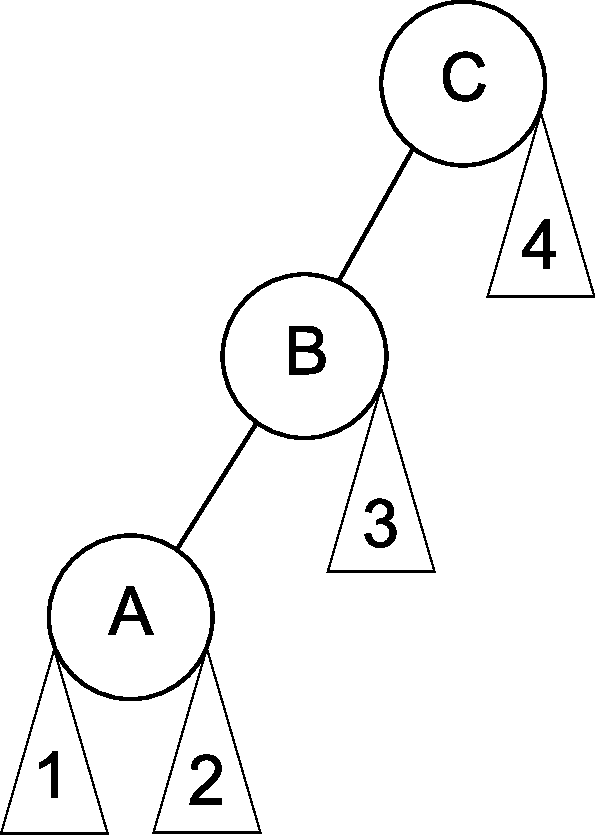
\includegraphics[width=.33\textwidth]{left_left.pdf}
\end{figure}


\subsection*{Right-Right}
\begin{figure}[h]
\centering
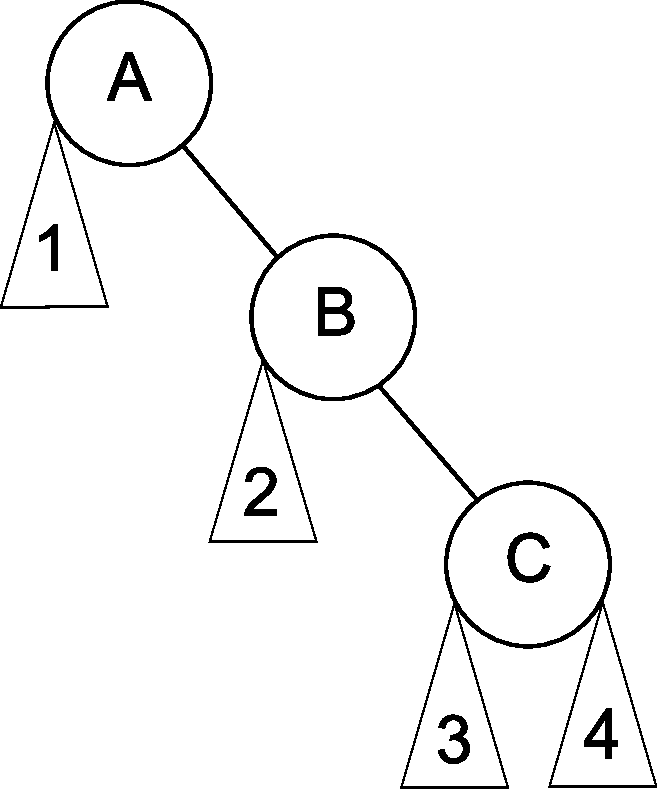
\includegraphics[width=.33\textwidth]{right_right.pdf}
\end{figure}

\subsection*{Left-Right}
\begin{figure}[h]
\centering
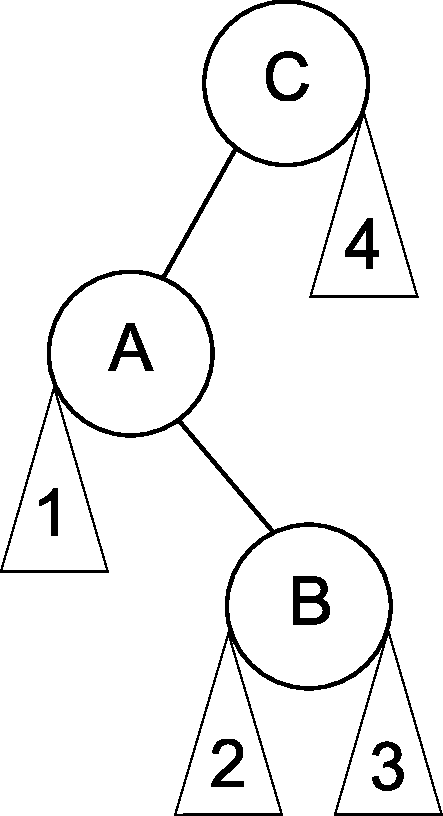
\includegraphics[width=.33\textwidth]{left_right.pdf}
\end{figure}

\subsection*{Right-Left}
\begin{figure}[h]
\centering
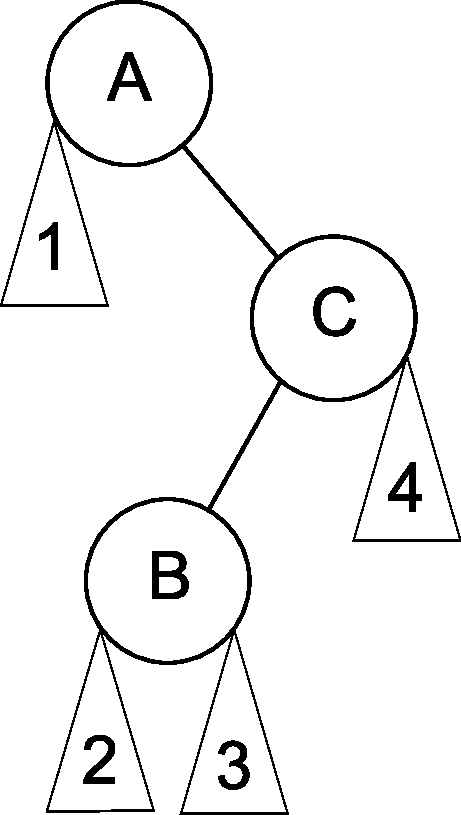
\includegraphics[width=.33\textwidth]{right_left.pdf}
\end{figure}
